% GNUPLOT: LaTeX picture with Postscript
\begingroup
  \makeatletter
  \providecommand\color[2][]{%
    \GenericError{(gnuplot) \space\space\space\@spaces}{%
      Package color not loaded in conjunction with
      terminal option `colourtext'%
    }{See the gnuplot documentation for explanation.%
    }{Either use 'blacktext' in gnuplot or load the package
      color.sty in LaTeX.}%
    \renewcommand\color[2][]{}%
  }%
  \providecommand\includegraphics[2][]{%
    \GenericError{(gnuplot) \space\space\space\@spaces}{%
      Package graphicx or graphics not loaded%
    }{See the gnuplot documentation for explanation.%
    }{The gnuplot epslatex terminal needs graphicx.sty or graphics.sty.}%
    \renewcommand\includegraphics[2][]{}%
  }%
  \providecommand\rotatebox[2]{#2}%
  \@ifundefined{ifGPcolor}{%
    \newif\ifGPcolor
    \GPcolortrue
  }{}%
  \@ifundefined{ifGPblacktext}{%
    \newif\ifGPblacktext
    \GPblacktexttrue
  }{}%
  % define a \g@addto@macro without @ in the name:
  \let\gplgaddtomacro\g@addto@macro
  % define empty templates for all commands taking text:
  \gdef\gplbacktext{}%
  \gdef\gplfronttext{}%
  \makeatother
  \ifGPblacktext
    % no textcolor at all
    \def\colorrgb#1{}%
    \def\colorgray#1{}%
  \else
    % gray or color?
    \ifGPcolor
      \def\colorrgb#1{\color[rgb]{#1}}%
      \def\colorgray#1{\color[gray]{#1}}%
      \expandafter\def\csname LTw\endcsname{\color{white}}%
      \expandafter\def\csname LTb\endcsname{\color{black}}%
      \expandafter\def\csname LTa\endcsname{\color{black}}%
      \expandafter\def\csname LT0\endcsname{\color[rgb]{1,0,0}}%
      \expandafter\def\csname LT1\endcsname{\color[rgb]{0,1,0}}%
      \expandafter\def\csname LT2\endcsname{\color[rgb]{0,0,1}}%
      \expandafter\def\csname LT3\endcsname{\color[rgb]{1,0,1}}%
      \expandafter\def\csname LT4\endcsname{\color[rgb]{0,1,1}}%
      \expandafter\def\csname LT5\endcsname{\color[rgb]{1,1,0}}%
      \expandafter\def\csname LT6\endcsname{\color[rgb]{0,0,0}}%
      \expandafter\def\csname LT7\endcsname{\color[rgb]{1,0.3,0}}%
      \expandafter\def\csname LT8\endcsname{\color[rgb]{0.5,0.5,0.5}}%
    \else
      % gray
      \def\colorrgb#1{\color{black}}%
      \def\colorgray#1{\color[gray]{#1}}%
      \expandafter\def\csname LTw\endcsname{\color{white}}%
      \expandafter\def\csname LTb\endcsname{\color{black}}%
      \expandafter\def\csname LTa\endcsname{\color{black}}%
      \expandafter\def\csname LT0\endcsname{\color{black}}%
      \expandafter\def\csname LT1\endcsname{\color{black}}%
      \expandafter\def\csname LT2\endcsname{\color{black}}%
      \expandafter\def\csname LT3\endcsname{\color{black}}%
      \expandafter\def\csname LT4\endcsname{\color{black}}%
      \expandafter\def\csname LT5\endcsname{\color{black}}%
      \expandafter\def\csname LT6\endcsname{\color{black}}%
      \expandafter\def\csname LT7\endcsname{\color{black}}%
      \expandafter\def\csname LT8\endcsname{\color{black}}%
    \fi
  \fi
    \setlength{\unitlength}{0.0500bp}%
    \ifx\gptboxheight\undefined%
      \newlength{\gptboxheight}%
      \newlength{\gptboxwidth}%
      \newsavebox{\gptboxtext}%
    \fi%
    \setlength{\fboxrule}{0.5pt}%
    \setlength{\fboxsep}{1pt}%
    \definecolor{tbcol}{rgb}{1,1,1}%
\begin{picture}(9060.00,4460.00)%
    \gplgaddtomacro\gplbacktext{%
      \csname LTb\endcsname%%
      \put(976,800){\makebox(0,0)[r]{\strut{}$50$}}%
      \csname LTb\endcsname%%
      \put(976,1446){\makebox(0,0)[r]{\strut{}$60$}}%
      \csname LTb\endcsname%%
      \put(976,2092){\makebox(0,0)[r]{\strut{}$70$}}%
      \csname LTb\endcsname%%
      \put(976,2739){\makebox(0,0)[r]{\strut{}$80$}}%
      \csname LTb\endcsname%%
      \put(976,3385){\makebox(0,0)[r]{\strut{}$90$}}%
      \csname LTb\endcsname%%
      \put(976,4032){\makebox(0,0)[r]{\strut{}$100$}}%
      \csname LTb\endcsname%%
      \put(1931,327){\makebox(0,0){\strut{}$0$}}%
      \csname LTb\endcsname%%
      \put(3179,327){\makebox(0,0){\strut{}$0.2$}}%
      \csname LTb\endcsname%%
      \put(4427,327){\makebox(0,0){\strut{}$0.4$}}%
      \csname LTb\endcsname%%
      \put(5675,327){\makebox(0,0){\strut{}$0.6$}}%
      \csname LTb\endcsname%%
      \put(6923,327){\makebox(0,0){\strut{}$0.8$}}%
      \csname LTb\endcsname%%
      \put(8171,327){\makebox(0,0){\strut{}$1$}}%
    }%
    \gplgaddtomacro\gplfronttext{%
      \csname LTb\endcsname%%
      \put(6842,983){\makebox(0,0)[l]{\strut{}Plain helper}}%
      \csname LTb\endcsname%%
      \put(6842,804){\makebox(0,0)[l]{\strut{}Same helper, fine-tuned}}%
      \csname LTb\endcsname%%
      \put(6842,625){\makebox(0,0)[l]{\strut{}Other methods}}%
      \csname LTb\endcsname%%
      \put(3485,3073){\makebox(0,0)[l]{\strut{}Qwen3-1.7B}}%
      \csname LTb\endcsname%%
      \put(3772,3621){\makebox(0,0)[l]{\strut{}Qwen3-8B}}%
      \csname LTb\endcsname%%
      \put(5345,2952){\makebox(0,0)[l]{\strut{}Reranker-0.6B}}%
      \csname LTb\endcsname%%
      \put(5788,4032){\makebox(0,0)[l]{\strut{}Reranker-8B}}%
      \csname LTb\endcsname%%
      \put(2551,1192){\makebox(0,0)[l]{\strut{}Qwen3-1.7B tuned}}%
      \csname LTb\endcsname%%
      \put(2722,2517){\makebox(0,0)[l]{\strut{}Qwen3-8B tuned}}%
      \csname LTb\endcsname%%
      \put(2744,787){\makebox(0,0)[l]{\strut{}Reranker-0.6B tuned}}%
      \csname LTb\endcsname%%
      \put(2844,2023){\makebox(0,0)[l]{\strut{}Reranker-8B tuned}}%
      \csname LTb\endcsname%%
      \put(3323,3926){\makebox(0,0)[l]{\strut{}gpt-oss-120b}}%
      \csname LTb\endcsname%%
      \put(3398,2766){\makebox(0,0)[l]{\strut{}Qwen3-30B}}%
      \csname LTb\endcsname%%
      \put(6667,3760){\makebox(0,0)[l]{\strut{}CAPMAS}}%
      \csname LTb\endcsname%%
      \put(5502,3515){\makebox(0,0)[l]{\strut{}CAPMAS retrained}}%
      \csname LTb\endcsname%%
      \put(3142,3773){\makebox(0,0)[r]{\strut{}Qwen3-4B}}%
      \csname LTb\endcsname%%
      \put(2395,2767){\makebox(0,0)[r]{\strut{}Qwen3-4B tuned}}%
      \csname LTb\endcsname%%
      \put(8096,3035){\makebox(0,0)[r]{\strut{}Everything}}%
      \csname LTb\endcsname%%
      \put(678,2383){\rotatebox{-270.00}{\makebox(0,0){\strut{}Tasks completed (\%)}}}%
      \csname LTb\endcsname%%
      \put(4926,104){\makebox(0,0){\strut{}Unneeded authority granted (0 = none, 1 = everything the delegator holds)}}%
    }%
    \gplbacktext
    \put(0,0){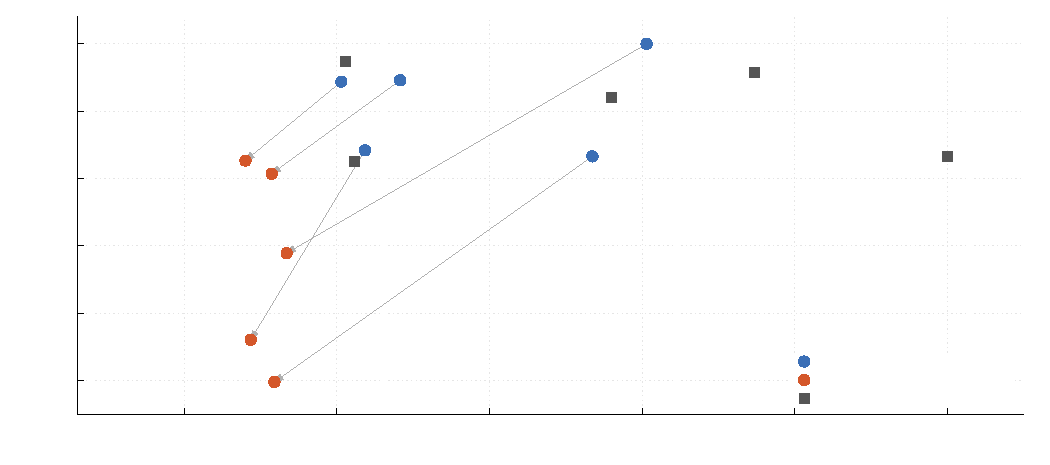
\includegraphics[width={453.00bp},height={223.00bp}]{figures/tradeoff}}%
    \gplfronttext
  \end{picture}%
\endgroup
